%appendix A
%p_update_manager

\section{Process: Update Manager}

\subsection{Visual}
\begin{figure}[ht]
    \centering
    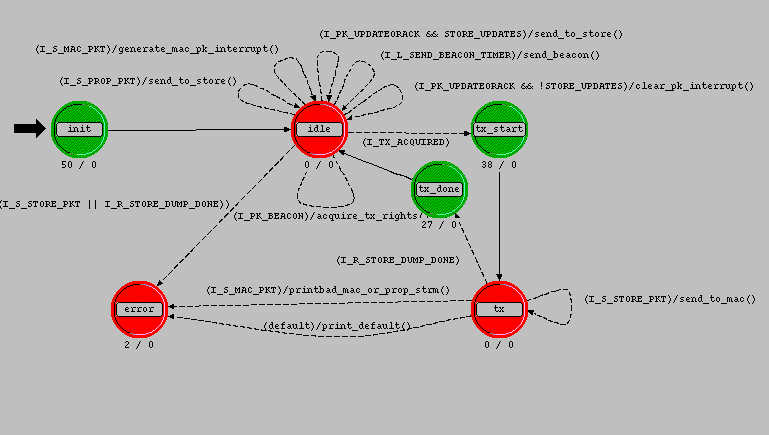
\includegraphics[width=.7\textwidth]{images/p_update_manager}
    \caption{Update manager process model}
    \label{fig:appendix-c}
\end{figure}

\subsection{Local variables}
\begin{figure}[ht]
    \centering
    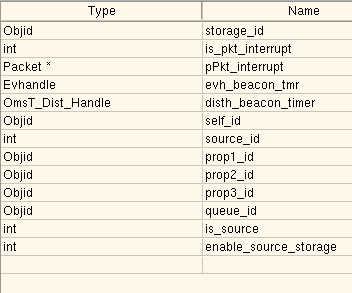
\includegraphics[width=.7\textwidth]{images/state_variable_update_manager}
    \caption{State variables of update manager process}
    \label{fig:appendix-c_sv}
\end{figure}

\subsection{Header Block}
%_____________________________________HEADER______________________________________
{\tiny
\begin{verbatim}
#include	<oms_dist_support.h>

//Streams
#define STRM_IN_P1		0
#define STRM_IN_P2		1
#define STRM_IN_P3		2
#define STRM_IN_STORE	3
#define STRM_OUT_STORE	0
#define STRM_IN_MAC		4
#define STRM_OUT_MAC 	1
//Interrupt Codes
#define IC_REQ_STORE_DUMP			73
#define IC_STORE_DUMP_DONE			74
#define IC_PROP_UPDATES_DISABLE		83
#define IC_PROP_UPDATES_ENABLE		84
#define IC_SEND_BEACON_TIMER		42
#define IC_PK_UPDATEORACK			37
#define IC_PK_BEACON				38
#define IC_Q_DISABLE				54
#define IC_Q_ENABLE					55
#define IC_TX_ACQUIRED				67
//Interrupts //Stream
#define I_S_PROP_PKT		(op_intrpt_type() == OPC_INTRPT_STRM && (op_intrpt_strm() == STRM_IN_P1 || op_intrpt_strm() == STRM_IN_P2 || op_intrpt_strm() == STRM_IN_P3))
#define I_S_STORE_PKT		(op_intrpt_type() == OPC_INTRPT_STRM && op_intrpt_strm() == STRM_IN_STORE)
#define I_S_MAC_PKT		(op_intrpt_type() == OPC_INTRPT_STRM && op_intrpt_strm() == STRM_IN_MAC)
//Packet op_intrpt_strm() == STRM_IN_P1
#define I_PK_UPDATEORACK	(op_intrpt_type() == OPC_INTRPT_SELF && op_intrpt_code() == IC_PK_UPDATEORACK)
#define I_PK_BEACON		(op_intrpt_type() == OPC_INTRPT_SELF && op_intrpt_code() == IC_PK_BEACON)
#define I_TX_ACQUIRED		((op_intrpt_type() == OPC_INTRPT_SELF || op_intrpt_type() == OPC_INTRPT_REMOTE) && op_intrpt_code() == IC_TX_ACQUIRED)
//Remote
#define I_R_STORE_DUMP_DONE	(op_intrpt_type() == OPC_INTRPT_REMOTE && op_intrpt_code() == IC_STORE_DUMP_DONE)
//Local (self)
#define I_L_SEND_BEACON_TIMER 	(op_intrpt_type() == OPC_INTRPT_SELF && op_intrpt_code() == IC_SEND_BEACON_TIMER)
//Other
#define STORE_UPDATES		(!is_source || enable_source_storage)

List *tx_rights_lst = OPC_NIL;
 
//PROTOTYPES
 
//Beacon control
void enable_beacon();
void disable_beacon();
void send_beacon();
void send_beacon_timed();
void reset_beacon_timer();
//Property control
void enable_prop_updates();
void disable_prop_updates();
void disable_q();
void enable_q();
//Storage control
void request_storage_dump();
//Packet redirection 
void send_to_store();
void send_to_mac();
void generate_mac_pk_interrupt();
void clear_pk_interrupt(void);
void printbad_mac_or_prop_strm(void);
void print_default(void);
void acquire_tx_rights(void);
\end{verbatim}
}

\subsection{Function Block}
%______________________________FUNCTION__________________________________
{\tiny
\begin{verbatim}
void schedule_beacon()
{
	double next_becon_time = 0;
	FIN(schedule_beacon());
	while(next_becon_time <= 0.1)
	{
		next_becon_time = oms_dist_outcome (disth_beacon_timer);
	}
	evh_beacon_tmr = op_intrpt_schedule_self (op_sim_time () + next_becon_time, IC_SEND_BEACON_TIMER);	
	FOUT;
}
void enable_beacon()
{
	FIN(enable_beacon());
	schedule_beacon();	
	FOUT;
}
void disable_beacon()
{
	FIN(disable_beacon());
	if (op_ev_valid (evh_beacon_tmr) == OPC_TRUE)
	{
		op_ev_cancel (evh_beacon_tmr);
	}
	FOUT;
}
void reset_beacon_timer()
{
	FIN(reset_beacon_timer());
	disable_beacon();
	enable_beacon();
	FOUT;
}
void send_beacon()
{
	char message_str[255];
	Packet *pPkt;
	FIN(send_beacon());
	pPkt = op_pk_create_fmt("beacon");
	op_pk_nfd_set_int32(pPkt, "source_id", source_id);
	op_pk_send(pPkt, STRM_OUT_MAC);
	schedule_beacon();	
	FOUT;
}
//Property control
void enable_prop_updates()
{
	FIN(enable_prop_updates());
	op_intrpt_schedule_remote(op_sim_time(), IC_PROP_UPDATES_ENABLE, prop1_id);
	op_intrpt_schedule_remote(op_sim_time(), IC_PROP_UPDATES_ENABLE, prop2_id);
	op_intrpt_schedule_remote(op_sim_time(), IC_PROP_UPDATES_ENABLE, prop3_id);
	FOUT;
}
void disable_prop_updates()
{
	FIN(disable_prop_updates());
	op_intrpt_schedule_remote(op_sim_time(), IC_PROP_UPDATES_DISABLE, prop1_id);
	op_intrpt_schedule_remote(op_sim_time(), IC_PROP_UPDATES_DISABLE, prop2_id);
	op_intrpt_schedule_remote(op_sim_time(), IC_PROP_UPDATES_DISABLE, prop3_id);	
	FOUT;
}
void request_storage_dump()
{
	FIN(request_sotrage_dump());
	op_intrpt_schedule_remote(op_sim_time(), IC_REQ_STORE_DUMP, storage_id);	
	FOUT;
}
void send_to_store()
{
	Packet *pPktToForward;
	FIN(send_to_store());
	if(is_pkt_interrupt)
	{
		is_pkt_interrupt = 0;
		if(pPkt_interrupt == OPC_NIL)
		{
			op_sim_end("Nill interrupt pkt", "", "", "");	
		}
		pPktToForward = pPkt_interrupt;
		pPkt_interrupt = OPC_NIL;
	}
	else
	{
		if(pPkt_interrupt != OPC_NIL)
		{
			op_sim_end("Not nill interrupt pkt", "", "", "");	
		}	
		pPktToForward = op_pk_get(op_intrpt_strm());
	}
	op_pk_send(pPktToForward, STRM_OUT_STORE);
	FOUT;
}
void send_to_mac()
{
	char message_str[255];
	Packet *pPktToForward;
	FIN(send_to_mac());
	if(is_pkt_interrupt)
	{
		is_pkt_interrupt = 0;
		if(pPkt_interrupt == OPC_NIL)
		{
			op_sim_end("Nill interrupt pkt", "", "", "");	
		}
		pPktToForward = pPkt_interrupt;
		pPkt_interrupt = OPC_NIL;
	}
	else
	{
		if(pPkt_interrupt != OPC_NIL)
		{
			op_sim_end("Not nill interrupt pkt", "", "", "");	
		}	
		pPktToForward = op_pk_get(op_intrpt_strm());
	}
	op_pk_send(pPktToForward, STRM_OUT_MAC);	
	FOUT;
}
void clear_pk_interrupt()
{
	FIN(clear_pk_interrupt());	
	if(is_pkt_interrupt)
	{
		is_pkt_interrupt = 0;
		if(pPkt_interrupt == OPC_NIL)
		{
			op_sim_end("Nill interrupt pkt", "", "", "");	
		}	
		op_pk_destroy(pPkt_interrupt);
		pPkt_interrupt = OPC_NIL;
	}
	else
	{
		op_sim_end("clear_pk_interrupt called wrong", "", "", "");	
	}	
	FOUT;
}
void generate_mac_pk_interrupt()
{
	char message_str[255];
	char format_name[255];
	FIN(generate_mac_pk_interrupt());
	reset_beacon_timer(); //To prevent a bad state

	if(pPkt_interrupt != OPC_NIL)
	{
		op_sim_end("Not nill interrupt pkt", "", "", "");	
	}
	else if (is_pkt_interrupt)
	{
		op_sim_end("Pkt interrupt flag set (bad)", "", "", "");		
	}
	else if(op_intrpt_strm() != STRM_IN_MAC)
	{
		op_sim_end("generate_mac_pk_interrupt called for non mac stream interrupt", "", "", "");	
	}
	pPkt_interrupt = op_pk_get(STRM_IN_MAC);
	is_pkt_interrupt = 1;
	op_pk_format (pPkt_interrupt, format_name);
	if (strcmp (format_name, "beacon") == 0)
	{
		op_intrpt_schedule_self(op_sim_time(), IC_PK_BEACON);	
	}
	else if (strcmp (format_name, "keyupdate") == 0)
	{
		op_intrpt_schedule_self(op_sim_time(), IC_PK_UPDATEORACK);	
	}	
	FOUT;
}
void disable_q()
{
	FIN(disable_q());
	op_intrpt_schedule_remote(op_sim_time(), IC_Q_DISABLE, queue_id);	
	FOUT;
}
void enable_q()
{
	FIN(enable_q());
	op_intrpt_schedule_remote(op_sim_time(), IC_Q_ENABLE, queue_id);	
	FOUT;
}
void print_default()
{
	FIN(print_default());
	printf("DEFAULT\n");
	FOUT;
}
void acquire_tx_rights()
{
	int i;
	FIN(acquire_tx_rights());
	
	if(is_pkt_interrupt)
	{
		is_pkt_interrupt = 0;
		if(pPkt_interrupt == OPC_NIL)
		{
			op_sim_end("Nill interrupt pkt", "", "", "");	
		}	
		op_pk_destroy(pPkt_interrupt);
		pPkt_interrupt = OPC_NIL;
	}
	else
	{
		if(pPkt_interrupt != OPC_NIL)
		{
			op_sim_end("Not nill interrupt pkt", "", "", "");	
		}
	}
	
	for(i = 0; i < op_prg_list_size(tx_rights_lst); i++)
	{
		if(op_prg_list_access(tx_rights_lst, i) == &self_id)
		{
			if(i = 0)
			{
				op_sim_end("NOOOOO.......", "", "", "");	
			}		
			FOUT;
		}
	}
	op_prg_list_insert(tx_rights_lst, &self_id, OPC_LISTPOS_TAIL);
	if(op_prg_list_size(tx_rights_lst) == 1)
	{
		op_intrpt_schedule_self(op_sim_time(), IC_TX_ACQUIRED);
	}
	FOUT;
}

\end{verbatim}
}
\subsection{Init State}
%______________________________________Init_____________________________________________________________
{\tiny
\begin{verbatim}
char beacon_dist_str[128];
self_id = op_id_self();
op_ima_obj_attr_get (self_id, "Source ID", &source_id);
op_ima_obj_attr_get (self_id, "Beacon Interval", beacon_dist_str);
disth_beacon_timer = oms_dist_load_from_string (beacon_dist_str);
op_ima_obj_attr_get (self_id, "Is Source", &is_source);
op_ima_sim_attr_get (OPC_IMA_INTEGER, "Enable Source Storage", &enable_source_storage);
storage_id = op_id_from_name (op_topo_parent(self_id), OPC_OBJTYPE_PROC, "storage");
prop1_id = op_id_from_name (op_topo_parent(self_id), OPC_OBJTYPE_PROC, "prop1");
prop2_id = op_id_from_name (op_topo_parent(self_id), OPC_OBJTYPE_PROC, "prop2");
prop3_id = op_id_from_name (op_topo_parent(self_id), OPC_OBJTYPE_PROC, "prop3");
queue_id = op_id_from_name (op_topo_parent(self_id), OPC_OBJTYPE_PROC, "hold_queue");
if(tx_rights_lst == OPC_NIL)
{
	printf("Creating TX rights list\n");
	tx_rights_lst = op_prg_list_create();
}
//Property stream priorities
op_intrpt_priority_set (OPC_INTRPT_STRM, STRM_IN_P1, 15);
op_intrpt_priority_set (OPC_INTRPT_STRM, STRM_IN_P2, 15);
op_intrpt_priority_set (OPC_INTRPT_STRM, STRM_IN_P3, 15);
//Lower than property inputs
op_intrpt_priority_set (OPC_INTRPT_STRM, STRM_IN_STORE, 10);
op_intrpt_priority_set (OPC_INTRPT_STRM, STRM_IN_MAC, 8);
//Absolute highest - controlled by stream interrupts
op_intrpt_priority_set (OPC_INTRPT_SELF, IC_PK_BEACON, 20);
op_intrpt_priority_set (OPC_INTRPT_SELF, IC_PK_UPDATEORACK, 20);
op_intrpt_priority_set (OPC_INTRPT_SELF, IC_TX_ACQUIRED, 20);
//Lower than STRM_IN_STORE
op_intrpt_priority_set (OPC_INTRPT_REMOTE, IC_STORE_DUMP_DONE, 9);
//Absolute lowest
op_intrpt_priority_set (OPC_INTRPT_SELF, IC_SEND_BEACON_TIMER, 0);
enable_beacon();
\end{verbatim}
}

\subsection{Active State}
%______________________________________Active_____________________________________________________________
{\tiny
\begin{verbatim}
Packet *pPkt;
if(prop_key_update_counter != prop_last_key_updated)
{
	active_update_tacker *pTracker;
	int i;
	
	//Error check
	for(i = 0; i < op_prg_list_size(active_updates_lst); i++)
	{
		//Might be able to just check the tail instead
	
		pTracker = (active_update_tacker *)op_prg_list_access(active_updates_lst, i);
		if(pTracker->update_counter_number == prop_last_key_updated)
		{
			if(pTracker->has_one_store == 0)
			{
				op_sim_end("Did not receive store interrupt", "", "", "");
			}
		}
	}
	prop_last_key_updated = prop_key_update_counter;
	pPkt = op_pk_create_fmt("keyupdate");
	op_pk_nfd_set_int32(pPkt, "source_id", source_id);		
	op_pk_nfd_set_int32(pPkt, "key", prop_key);	
	op_pk_nfd_set_int32(pPkt, "key_update_number", prop_key_update_counter);
	op_pk_nfd_set_dbl(pPkt, "generated_timestamp", op_sim_time());
	op_pk_nfd_set_objid(pPkt, "source_prop_objid", self_id);
	pTracker = (active_update_tacker *) op_prg_mem_alloc (sizeof (active_update_tacker));
	pTracker->update_counter_number = prop_key_update_counter;
	pTracker->pkts_alive = 0;
	pTracker->has_one_store = 0;
	pTracker->gateway_rx = 0;
	pTracker->generated_timestamp = op_sim_time();
	pTracker->mark_for_delete = 3;
	op_prg_list_insert(active_updates_lst, pTracker, OPC_LISTPOS_TAIL);	
	op_pk_send(pPkt, 0); //Output stream
}
\end{verbatim}
}

\subsection{tx_start State}
%_____________________________________tx_start____________________________________________________________
{\tiny
\begin{verbatim}
if(op_prg_list_access(tx_rights_lst, OPC_LISTPOS_HEAD) != &self_id)
{
	op_sim_end("Dont have TX rights", "", "", "");	
}
if(is_pkt_interrupt)
{
	is_pkt_interrupt = 0;	
	if(pPkt_interrupt == OPC_NIL)
	{
		op_sim_end("Nill interrupt pkt", "", "", "");	
	}		
	op_pk_destroy(pPkt_interrupt);
	pPkt_interrupt = OPC_NIL;
}
else
{
	if(pPkt_interrupt != OPC_NIL)
	{
		op_sim_end("Not nill interrupt pkt", "", "", "");	
	}
}
if(op_pk_get(STRM_IN_MAC) != OPC_NIL)
{
	op_sim_end("STRM_IN_MAC - Packet waiting", "", "", "");	
}
disable_q();
disable_prop_updates();

disable_beacon();
request_storage_dump();

\end{verbatim}
}